\documentclass[12pt]{article}
\usepackage[utf8]{inputenc}
\usepackage[T1]{fontenc}
\usepackage{amsmath,amsfonts,amssymb}
\usepackage{graphicx}
\usepackage{a4wide}
\usepackage{hyperref}
%\usepackage[style=numeric-comp]{biblatex}
\usepackage{enumerate}

\newcommand{\D}{{2^Q}}
\newcommand{\bw}{\mathbf{w}}
\newcommand{\bwT}{\mathbf{w}^\mathsf{T}}
\newcommand{\T}{^\mathsf{T}}
\newcommand{\bphi}{\boldsymbol{\varphi}}
\newcommand{\bx}{\mathbf{x}}
\newcommand{\bc}{\mathbf{c}}
\newcommand{\bd}{\mathbf{d}}
\usepackage{graphicx}
\usepackage{wrapfig}
\usepackage{subcaption}

\begin{document}
\begin{center}
{\Huge\bf Collided birthdays are welcome!}
\end{center}
%\author{Vadim Strizhov}%\footnote{E-mail: vadim.vct@gmail.com}}

\begin{quote}
Multiple radio-frequency data transmitters often collide in one time-slot. We describe ways to detect the collisions. The good news: no matter the collision, the transmitters could be identified and data could be restored. It significantly ameliorates the radio-frequency identification systems.\footnote{Vadim Strizhov, \href{mailto:vadim.vct@gmail.com}{\texttt{vadim.vct@gmail.com}}, 18/03/2025}

\bigskip
\noindent \textbf{Keywords:} machine learning; aloha collision; collision detection; self-modeling regression; additive regularization
\bigskip
\end{quote}

\section{Collision-free inventory}
Imagine an overloaded shopping cart. We need to scan all items at one go. Each item has its ID radio tag. At the counter all tags are called and all tags are replied.  
\begin{wrapfigure}{r}{0.3\textwidth}  %
%\begin{figure}[!tb]
\centering
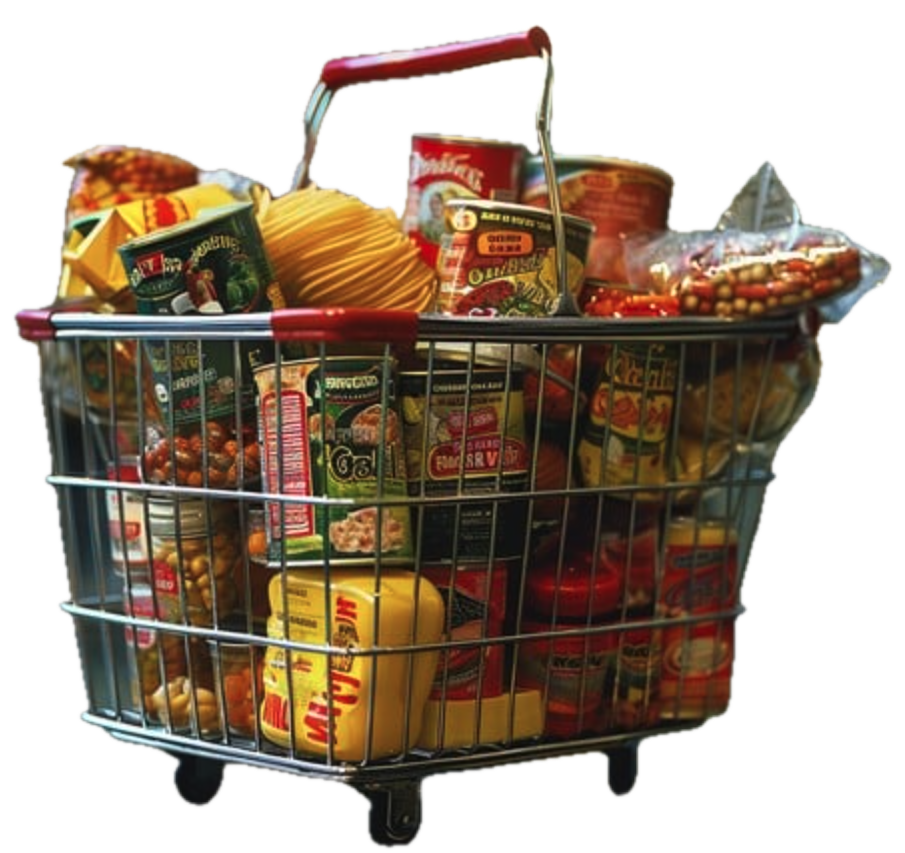
\includegraphics[width=\linewidth]{fig_shopping-cart}
\caption{The goal is to inventory over 1,000 tags at once.}
\label{fig:pr_p0}
%\end{figure}
\end{wrapfigure}
The Aloha protocol resolve mixture of replies: the inventory time-segment splits into time-slots. At request each tag waits a random number of time slots and reply. Due this randomness, some  time slots left  unoccupied, some time slots keep a single tad ID, but some still occupied by several tags. Can we avoid collisions in one inventory cycle? The problem of estimation of probability that two tags hit one slot is called \emph{the birthday paradox}~\cite{Santos2015,Mosteller1962}. What is probability of a two people have their birthdays in the same day? One tag hits any of~$D$ slots with the probability of~$\frac{1}{D}$. Two tags do not hit the same slot with the probability~$1-\frac{1}{D}$. The third tag cannot hit the both occupied slots so the probability is
\[
\frac{D-1}{D} \frac{D-2}{D} = \left(1-\frac{1}{D}\right) \left(1- \frac{2}{D}\right).
\] 
So for given~$D$ slots,  the probability that none of~$N$ tags do not collide is
\[
\frac{D!}{D^N(D-N)!}.
\] 
Figure~\ref{fig:pr_collision-free} shows that the probability of successful inventory is small for any reasonable number of tags. So if the shopping cart has over 100 items with tags, most likely there is collision even for a long inventory cycle. See the green and red lines. 
\begin{figure}[!tb]
\centering
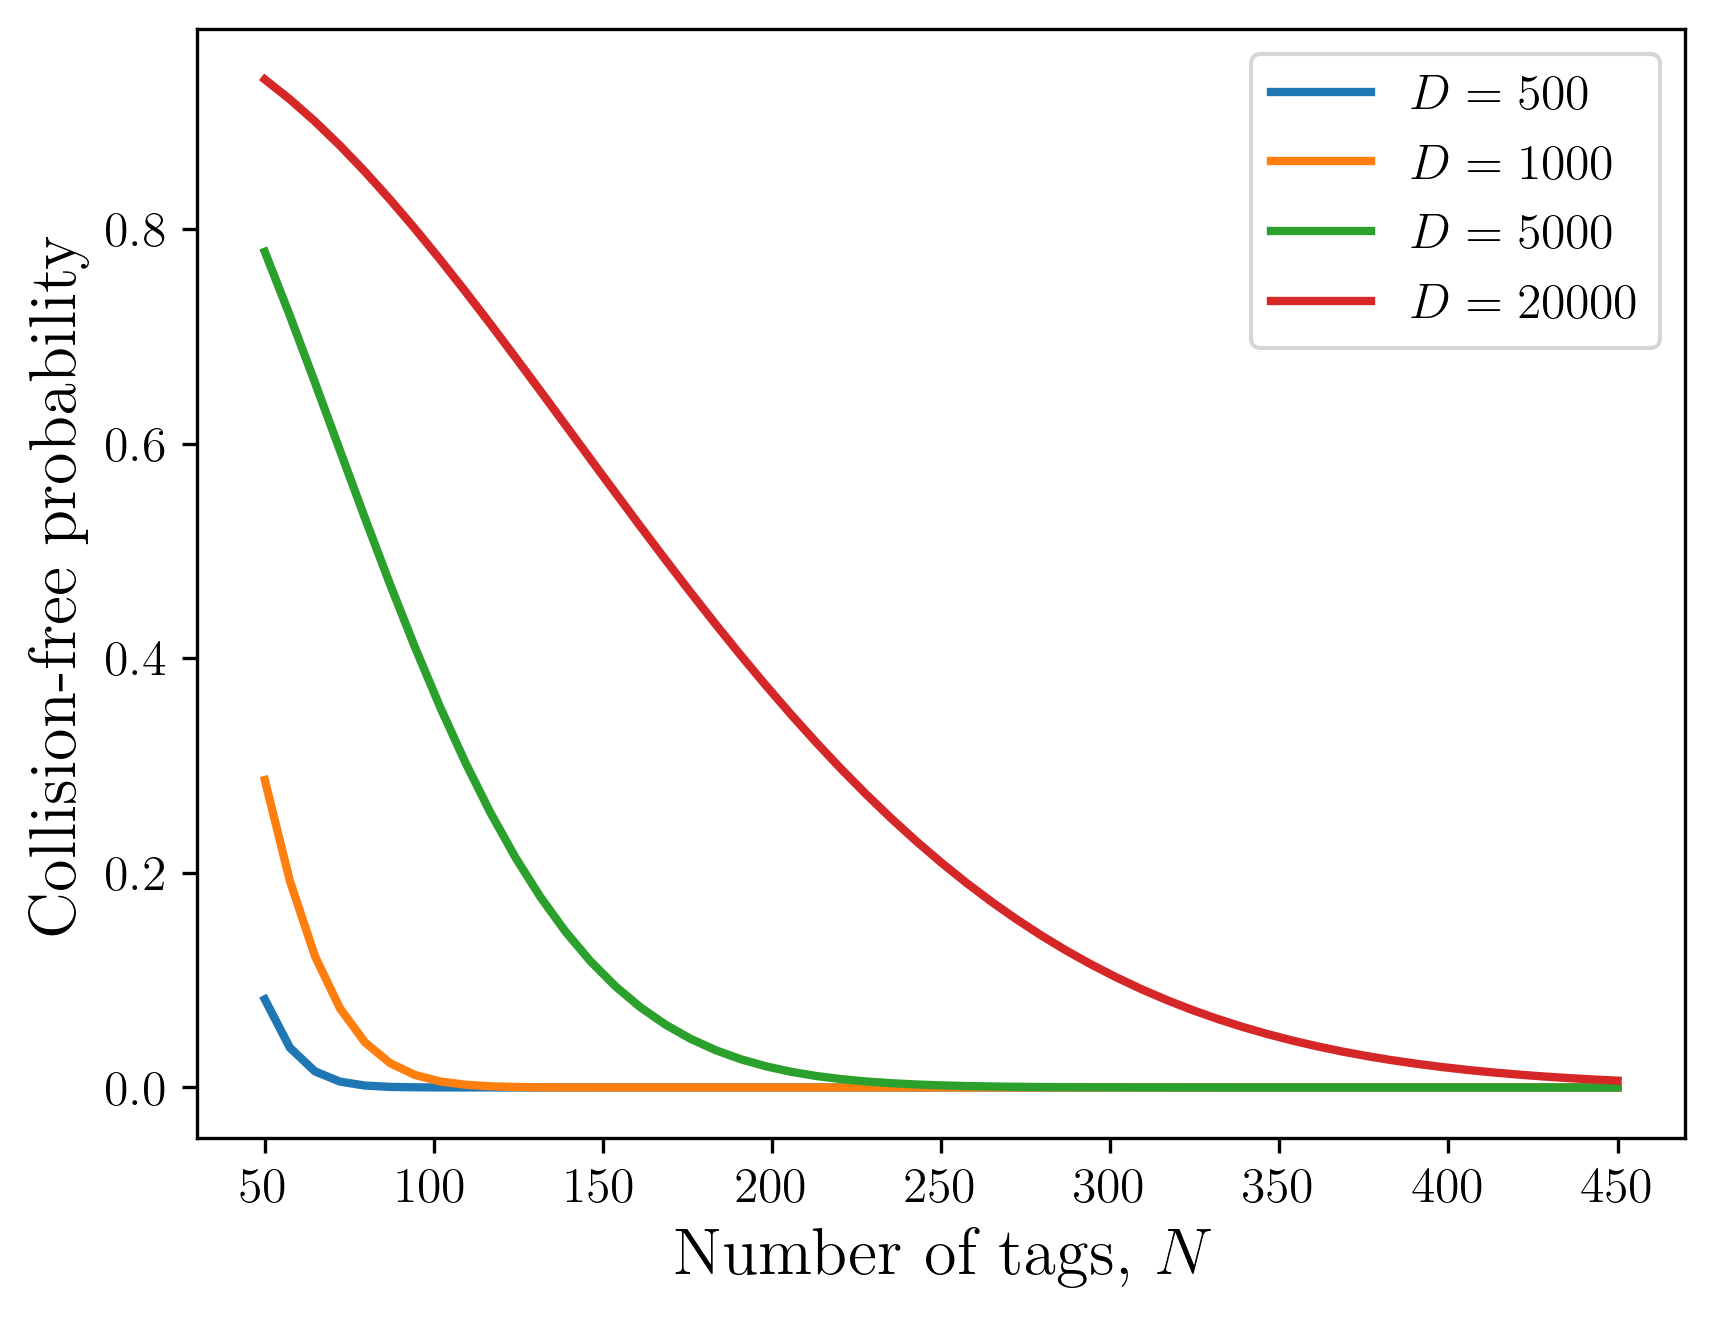
\includegraphics[width=0.6\textwidth]{fig_collision_free}
\caption{The probability of collision-free inventory of any of $N$ given $D$ time-slots.}
\label{fig:pr_collision-free}
\end{figure}

If, with an insufficiently small number of slots, there is no initial period where the probability of getting two transmitters in one slot increases. That is, if there are enough transmitters to overlap at all, they will \emph{immediately start crowding} into multiple transmissions per slot.

Briefly, \emph{the collision is inaviodable in one inventory cycle.}
%Though the probability of collision of many tags is relatively insignificant, the probability of experience a collision during a single inventory cycle is real thing and it makes our main question important. 

\section{Signal self-modeling}
The collision should be detected to avoid inventory errors. But there is no error in signals, reconstructed after collision. So we suppose two or more tags transmit at the same time. 
\begin{wrapfigure}{r}{0.2\textwidth}  %\begin{figure}[!tb]
\centering
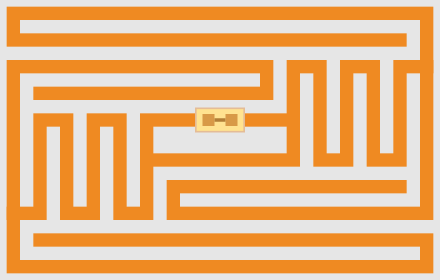
\includegraphics[width=\linewidth]{EPC-RFID-TAG.svg.png}
\caption{A tag emits an ultra-high-frequency signal through its antenna.}
\label{fig:antenna}%\end{figure}
\end{wrapfigure}
The inventory reader decodes the high-frequency signal into the I/Q data signal (In-phase/Quadrature). This signal carries two time series, real and imaginary. Denote these time series by~$\mathbf{x}$, a vector in the complex space. 

Since the tags are located in the different parts of shopping cart its signal is varied by phase and amplitude. Figure~\ref{fig:projected_shift} shows the same signal with the phase and amplitude modifications. The self-regression model approximates these signals with only two parameters: scale and shift.

\begin{figure}[!tp]
\centering
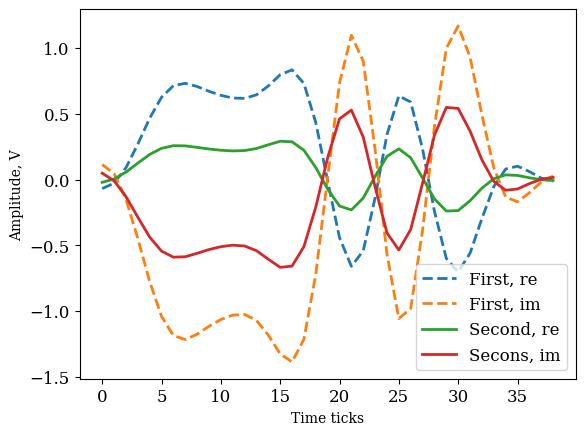
\includegraphics[width=0.45\textwidth]{fig_amplitude_scaled_distance}
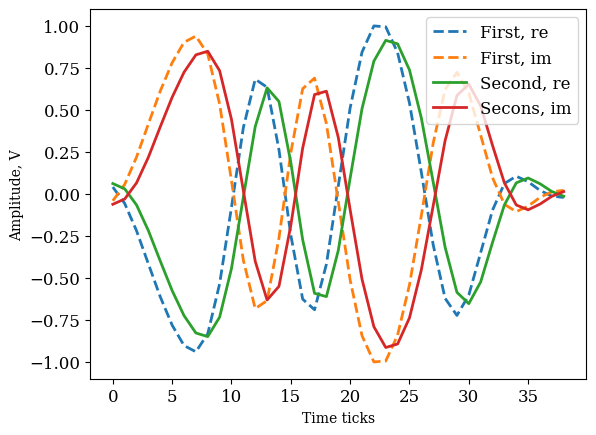
\includegraphics[width=0.45\textwidth]{fig_centroid_still_in_cluster}
\caption{The self-modeling regression regresses first signal to second (left), while shifting the phase of the whole I/Q data signal to find the best fit (right). The legend shows real and imaginary parts of the complex signal.}
\label{fig:projected_shift}
\end{figure}

The self-modeling regression. It approximates the signal~$\bx$ with the standard signal~$\bc$ (call it the centroid) as
\[
\hat{\bc} = \text{scale} \cdot \bigl( \text{shift}(\bx)\bigr),
\]  
%\hat{\bc} = v_1 \bigl( \text{shift}(\bx, v_2)\bigr),
with two scalar parameters: scale and shift. The first parameter is calculated as the dot product ratio of the projection 
\[
\text{scale}\cdot \bx = \frac{\bc\T\bx}{\|\bc\|^2}\bc.
\]
%Note that this ratio could be negative, which is an admissible operation for the I/Q data signal. 
The second parameter calculated as an argument of minimum distance
\[
\text{shift} =\mathop{\arg\min}\|\hat{\bc}-\bc\|^2.
\]
%For the simplicity of the computations and signal processing procedures, most part of the model acts in the complex space. The variables $\bx, \bd, \bc \in \mathbb{C}^T$, where~$T$ is the length of the transmitted I/Q data signal,  $\bphi, \bw \in \mathbb{R}^K$, where~$K$ is the number of centroids, and the class~$y\in\{0,1\}.$ The in-phase part of the complex vector~$\bx$ is real, while the quadrature part is imaginary.

%Figure~\ref{fig:projected_shift} illustrates the self-modeling regression. The first, dashed, signal is the centroid, scaled to 1\,V, and the second, solid, signal is modified to approximate the centroid.

The result of self-modeling is shown in Figure~\ref{fig:cluster}
\begin{figure}[!tp]
\centering
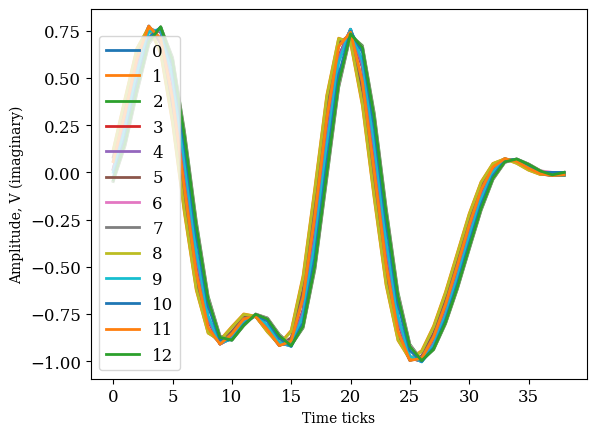
\includegraphics[width=0.45\textwidth]{fig_cluster}
\caption{After the self-modeling regression twelve different transmissions became similar (imaginary part is shown).}
\label{fig:cluster}
\end{figure}
\begin{figure}[!h]
\centering
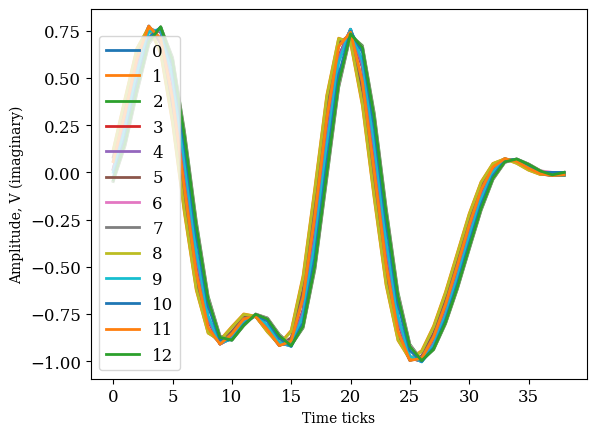
\includegraphics[width=0.5\textwidth]{fig_cluster}
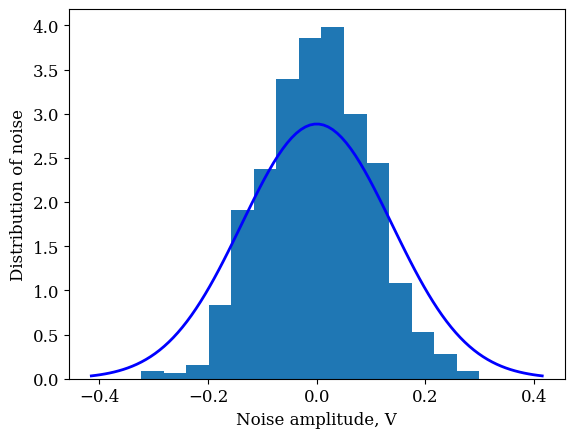
\includegraphics[width=0.45\textwidth]{fig_noise_pdf}
\caption{The left part of figure shows the cluster of transmitted signals with the same message without noise. They scaled to the same shift phase and amplitude.  The ground truth noise (right part), samples from the dataset, has $\mu\leq 0.005$ (real or image) and standard deviation~$\sigma =  0.1361$. The plot shows~$3 \sigma$. This distribution function us used in the $\geq 3$ signal reconstruction procedure. }  % mu 0.005097450126825286-9.32958204652807e-05j) sigma: 0.13612418396736398
\label{fig:demo}
\end{figure}

Briefly, \emph{self-modeling unifies the signal shape} of  I/Q data and it makes it a tool to analyze the signal mixtures. 

\newcommand{\bX}{\mathbf{X}}
\newcommand{\bv}{\mathbf{v}}
\newcommand{\bp}{\mathbf{p}}
\newcommand{\by}{\mathbf{y}}
\newcommand{\beps}{\boldsymbol{\epsilon}}

\section{Signal reconstruction}
When two and more tags hit the same time-slot their signals mixture. Suppose, due to the various antenna orientations, they mixture with different coefficients. For~$n$ tags denote the coefficients~$[v_1, \dots, v_n]$. The mixture~$\by$ comes as a signal
\[
\by = v_1 \bx_1 + \dots + v_n \bx_n = \bX\bv.
\] 
Here the columns of the matrix~$\bX$ are the stacked I/Q data signals. 
The coefficients~$\bv$ and their number~$n$ are unknown. But for any mixture coefficients, the signals of collided tags are in the subspace of the space of the matrix~$\bX$. Using the self-regression model, find the source signals as the nearest linear combination tho the received mixture, see Figure~\ref{fig:lsq}. 
\begin{figure}[!t]
\centering
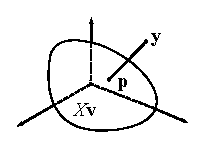
\includegraphics[width=0.2\textwidth]{fig_LeastSquaresProjection}
\caption{Two and more signals, mixture proportionally their attenuation, defines the vector span in the space of I/Q data signals. Here the vector~$\bv$ is the weights of the linear combinations of the signals. The vector~$\bp$ is the orthogonal projection to the span~$\bX\bv$. The vector~$\by$ is the mixture of signals and the added noise to be reconstructed. The basis of~$P$ independent (the transmitters can not send the same data) I/Q data 
signals~$\bx_1,\ldots,\bx_P$ form the matrix~$\bX=[\bx_1,\ldots,\bx_P]$ as its columns.}
\label{fig:lsq}
\end{figure}
There is no need to use methods like blind signal separation. The self-modeling regression works even for a single-antenna reader. 

\begin{figure}[!htbp]
\centering
%\includegraphics[width=0.2\textwidth]{}
\caption{Each line is the number of successfully recognized IDs of the tags after the signal reconstruction. The x-axis shows level of noise from the expected standard deviation to zero. The y-axis shows the proportion (or number TODO) of randomly generated data.}
\label{fig:reconstruction}
\end{figure}
Figure~\ref{fig:reconstruction} shows that the most expected types of collision: two and three tags hit the same slot. It delivers good TODO I/Q data identity reconstruction.

Briefly, \emph{collision does not matter for the reconstructed signals}. 

\section{Collision detection}
After the reconstruction the collision detection sounds as a trivial problem.

The proposed collision detection classifier model is the superposition of logistic regression, radial basis functions with Gaussian kernels, and self-modeling regression. The first part returns the probability of collision as
\[
p(y|\bw) =\bigl( 1+\exp(-\bwT\bphi(\bx)) \bigr)^{-1}.
\]
The second part is the vector function~$\bphi(\bx)$ with Gaussian kernels 
\[
\bphi = [\varphi_1,\ldots,\varphi_K]\T, \quad \text{where} \quad \varphi_k(\bx) =  \exp\left(-\frac{\|\bd(\bx, \bc_k) - \bc_k\|^2}{2\sigma_k^2}\right).
\]
And the last part is 




%%%%%%%%%%%%%%%%%% TODO
So most likely, \emph{here is a way to read several tags with the same time-slot transmission.}
\section{?}
What is the probability of a collision of many items?t
%%%%%%%%%%%%%%%%%% TODO




\section{The dataset creation}
The signal mixture procedure is organized as follows. The initial data seems to be scaled already and the scale does not always follow the amplitude in the $0.3,\ldots,1.1$\,V segment. However, the signal at the given scaling seems decent. The same with the noise. Its level is assumed to be properly set, so we leave it unchanged. The signal of small energy will express a bigger influence of the noise at the reader, so unchanging the given settings seems to be a natural decision. 

Adding the signal increases their power for the same-phase case. To make the problem a little bit harder (signal attenuates with distance) we set the summing coefficients less than one: $0.5,\ldots,0.8$ fixing them for the experiment. The scaling \[A_\text{result} = \left| \sum_{i=1}^{N} A_i \exp({j\phi_i}) \right|,\] where $A$ are the amplitudes of the signals and $\phi$ is the phase difference between them~\cite{Balanis2005} (we find this with Gilbert transform, if the model complexity allows)  requires additional discussion.

The generated data sample size. Decoupling indexes of data and noise datasets and assuming that the mixture of Gaussian noise is the Gaussian noise with zero expectation could provide us with a big sample size. We set the size of the original data for each of the four classes.  In the case of~$\geq 3$ classes the mixture of 3 to five signals was generated.

\section{The classifier accuracy analysis}

Since the logistic regression model returns the probability of collision, the Area Under ROC is assigned as the quality criterion. For various cross-validations, its expected value is 9.7. For various normally-balanced datasets, it varies in the segment~$0.94,\ldots,0.98$. This means there is a reasonable probability of Aloha collision detection for one versus two or more transmitters. 

Since the Aloha collision detection is the main goal of this experiment, and since the noise detection is the essential part of signal analysis, we suggest to analyze the classifier accuracy for the following combinations:
1) noise versus all, 2) single transmitter versus two transmitters, 3) single transmitter versus two or three or more transmitters, and 4) two transmitters versus three or more transmitters. 

The problem of 2 versus $\geq 3$ transmitters \emph{with complete separation and reconstruction} of both collided signals is feasible for the given data. Figure~\ref{fig:AUC_1v2} shows the classification accuracy AUC = 0.67 without the reconstruction part; the latter is discussed in section~\ref{ICA}.

\begin{figure}[!tb]
\centering
%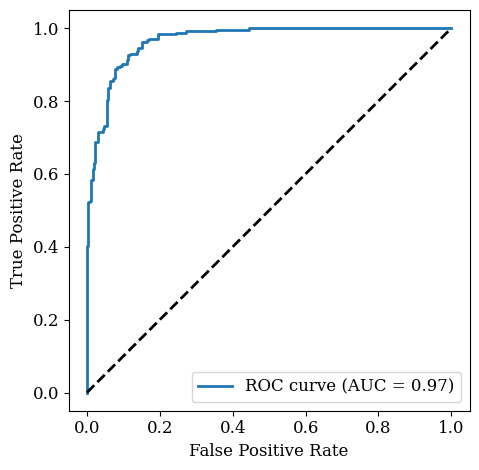
\includegraphics[width=0.32\textwidth]{fig_ROC_1v2}
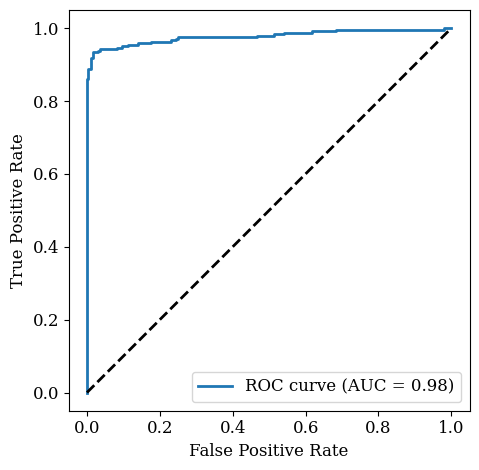
\includegraphics[width=0.32\textwidth]{fig_feb12_AUC_1vs2}
%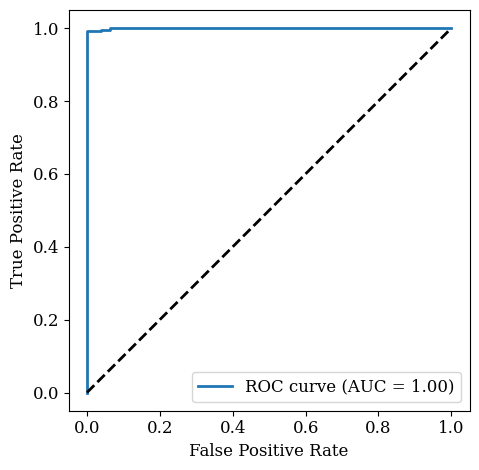
\includegraphics[width=0.32\textwidth]{fig_AUC_0vs1}
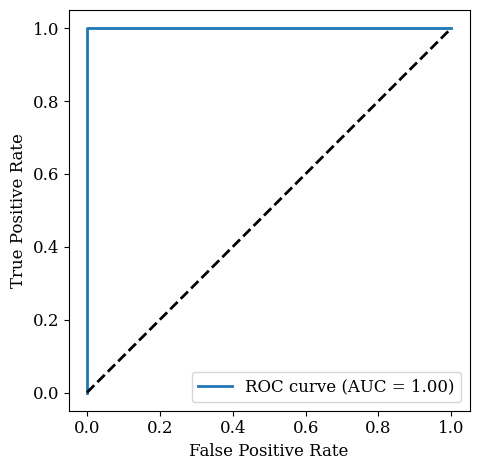
\includegraphics[width=0.32\textwidth]{fig_feb12_AUC_0vs123}\\
%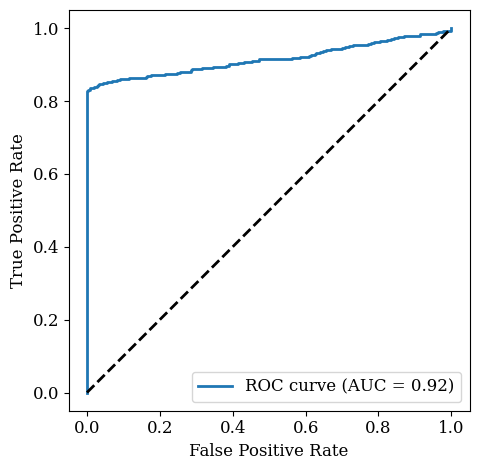
\includegraphics[width=0.32\textwidth]{fig_AUC_0vs123}\\
% 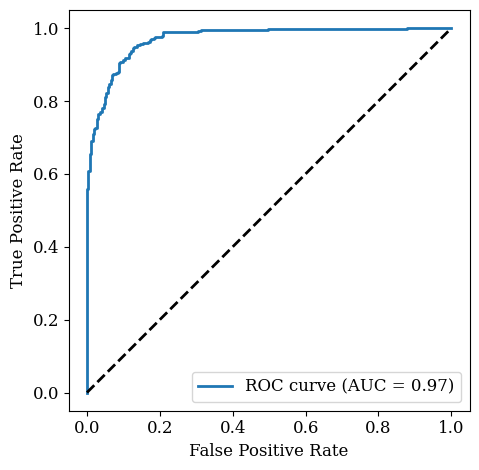
\includegraphics[width=0.32\textwidth]{fig_AUC1vs23}
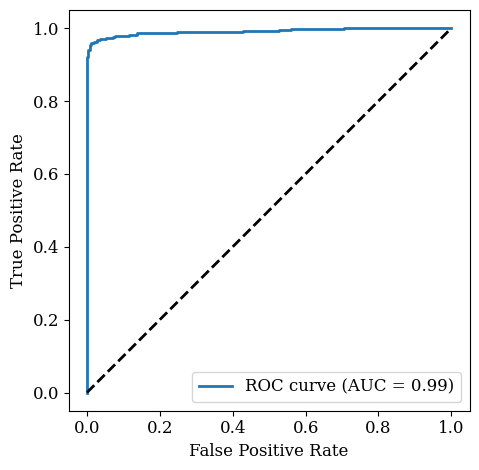
\includegraphics[width=0.32\textwidth]{fig_feb12_AUC_1vs23}
%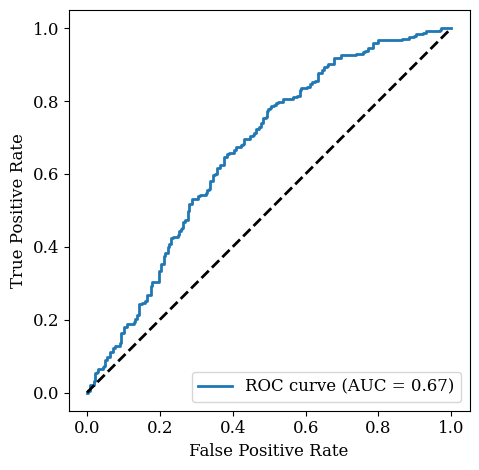
\includegraphics[width=0.32\textwidth]{fig_AUC_2vs3}
%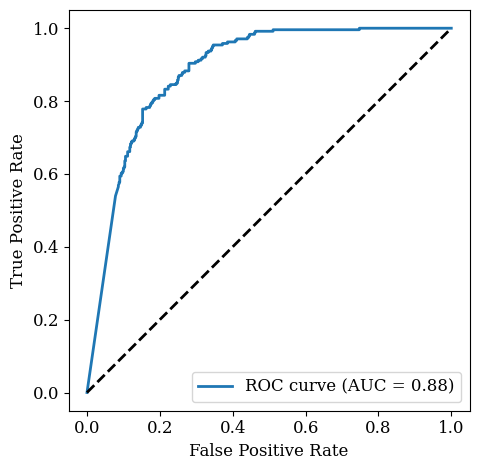
\includegraphics[width=0.32\textwidth]{fig_feb12_AUC_12vs3}
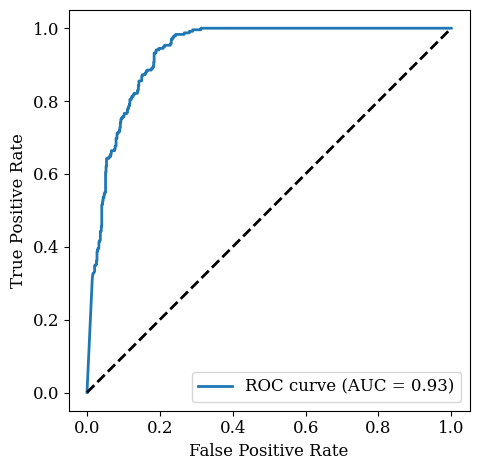
\includegraphics[width=0.32\textwidth]{fig_feb12_AUC_012vs3}
\caption{The model returns the probability of collision detection. The higher Operator Reciever Curve shows the better quality of detection (one transmitter versus two) on the \emph{test part} of the dataset.
The top row is 
1 versus 2 (left), %noise versus 1 (center), 
noise versus all (right). 
The bottom row is 1 versus 2 or $\geq3$ (left), and 
0, 1 or 2 versus $\geq3$ transmitters (right).
}
\label{fig:AUC_1v2}
\end{figure}

Interesting case for the classes 1 versus~$0,2,\text{or}\geq3$ when the RBF with logistic regression delivers~$\text{AUC}=0.66$ with two-hunch ROC curve, while kNN delivers~$\text{AUC}=0.96$ and accuracy~$0.97$. This case requires modification for the noise class, though the noise classification is straightforward with ~$\text{AUC}=1.0$ on the test noise versus all classes.

Figure~\ref{fig:AUC_1v2} shows the accuracy for the classification of a single transmitter versus the collision of two transmitters. The overall classification procedure is organized in the following way. The one-versus-all four classes classification problem is listed according to their probability: empty versus any transmission, one versus two transmitters, one versus two or more transmitters. The detection of three or more against two or more requires the blind signal separation procedure, which is introduced in Section~\ref{ICA}.

\section{Maximizing the accuracy on prior knowledge of $N,Q$}

Assume as the prior knowledge 1)~that the sufficient number of allocated for transmission time slots~$2^Q$ brings a small number of collisions of two and a lesser number of collisions of~$\geq 3$ transmitters and, 2)~the model parameters are subject to optimization during the reader's session. In this case, we suggest using predefined optimal parameters~$\bw_\text{opt}$, suitable for the current session or environment. For the model parameter optimization, apply a Bayesian penalty function for the current model. According to the Bayes' rule
\[
p(\bw|y,\bx) \propto p(y|\bw,\bx) p({\bw}_\text{opt}),
\]
it changes the most likely parameters~$p(y|\bw,\bx)$ for the most probable parameters~$p(\bw|y,\bx$. So the optimization criterion is 
\[
\mathcal{L}= \sum_{i=1}^m \biggl( y_i \log p(\bx_i,\bw) + (1-y_i) \log\bigl(1-p(\bx_i, \bw)\bigr)\biggr)+ \frac{1}{2}(\bw-\bw_\text{opt})\T\mathbf{A}^{-1}(\bw-\bw_\text{opt}).
\]
The covariance matrix~$A$ is estimated in the multiple cross-validation procedure using prior knowledge datasets. The \texttt{LogisticRegression} model from \texttt{sklearn} has the regularization component (the right part of this formula)  with~$\bw_\text{opt}=\boldsymbol{0}$ and $\mathbf{A} = \alpha\mathbf{I}$ by befault. 

Test the suggested collision classifier model on datasets with various sample sizes and class balance ratios. 
The approximate parameters for~$N$ and~$Q$ simulation were taken from the paper~\cite{Kang2011}. So let the number of single transmissions varies from 100 to 1000, and the ratio of collided transmission varies from 0.1 to 0.9.

\begin{figure}[!htbp]
\centering
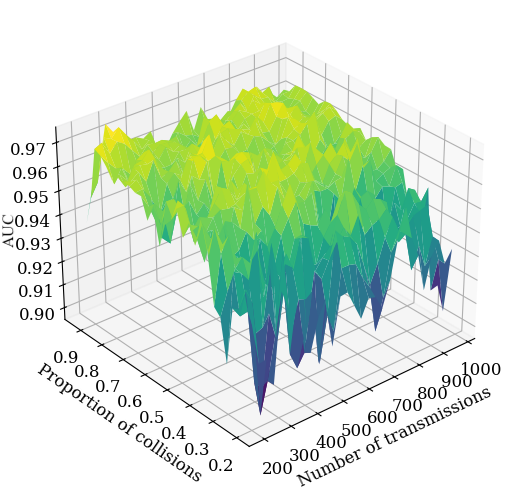
\includegraphics[width=0.49\textwidth]{fig_sampe_size_mean2}
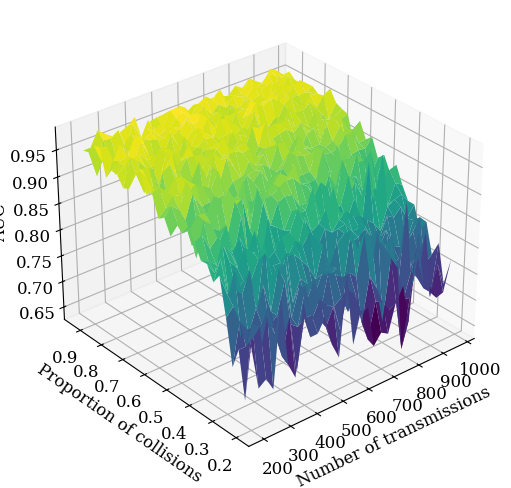
\includegraphics[width=0.49\textwidth]{fig_sampe_size_kNN}
\caption{The accuracy of collision detection depends on the dataset sample size and class imbalance. The z-axis shows AUC. The left part is 1 versus two transmitters with logistic regression model, the right part is 1 versus 2 and $\geq 3$ transmitters with kNN model.}
\label{fig:samle_size}
\end{figure}

Figure~\ref{fig:samle_size} illustrates \emph{the class balancing} problem. It shows that the accuracy is stable around borderline values of the sample size and class balance ratio. It varies in the segment~$0.90,\ldots,0.97$ for training data. Each point of the surface is an independent train-test cycle for the regression model. The right axis shows the sample size for the single-transmission class. The left axis shows the proportion of this value in the collision class. So the summary of these two values makes the size of the dataset. 

Since to optimize the model parameters we use the Newton-Raphson algorithm~\cite{Motrenko2014} that has small computational complexity and has good convergence to the optimal parameters, it could be ported to the reader. In this case, we suggest using the optimization criterion~$L$ to improve the imbalance of classes.  

However, this suggested model has equal centroids according to the assumption that different transmitters has equal probability to act on the reader's request. So we suggest to fix the parameters of the model to their equal values. In this case, there is no need to optimize the model parameters in the reader. 

\section{Model portability analysis}
To classify one transmitted signal the model uses the following operations:
\begin{enumerate}[1)]
\item projection \texttt{complex}: $K \times T \times 2S$ multiplications,
\item shifting \texttt{complex}: $K \times T \times 2S$ additions,
\item distance  \texttt{complex}: $K \times T$ additions and multiplications,
\item classification \texttt{float}: $T$  multiplications,
\item not counting single operations and padding,
\item there is \texttt{float}: $K+1$ exponent operations.
\end{enumerate}
Assuming the number of centroids~$K=128$, the length of the I/Q data signal $T=39$, and the admissible phase shift parameter is~$\pm$ time ticks, $S=10$. % 2*K*T*S+K*T. 
With a single projection procedure~$S=1$, it takes $128\times 39 \times 2$ operations. In this case the expected \mbox{$\text{AUC}=9.3$}. However, without significant loss of accuracy, we could downsample I/Q data to the required number of operations. Providing the Gaussian noise expectation is zero, no denoising and additional operations are required. Also, since the logistic regression model parameters are assumed to be equal, we can classify the values of the kernel function by threshold. 
The model requires memory \texttt{complex}: $128\times 39$. % Memory for for ~$\geq 3$ classes takes~$128^2*39.$ 
These estimations are preliminary. 


\begin{figure}[!h]
\centering
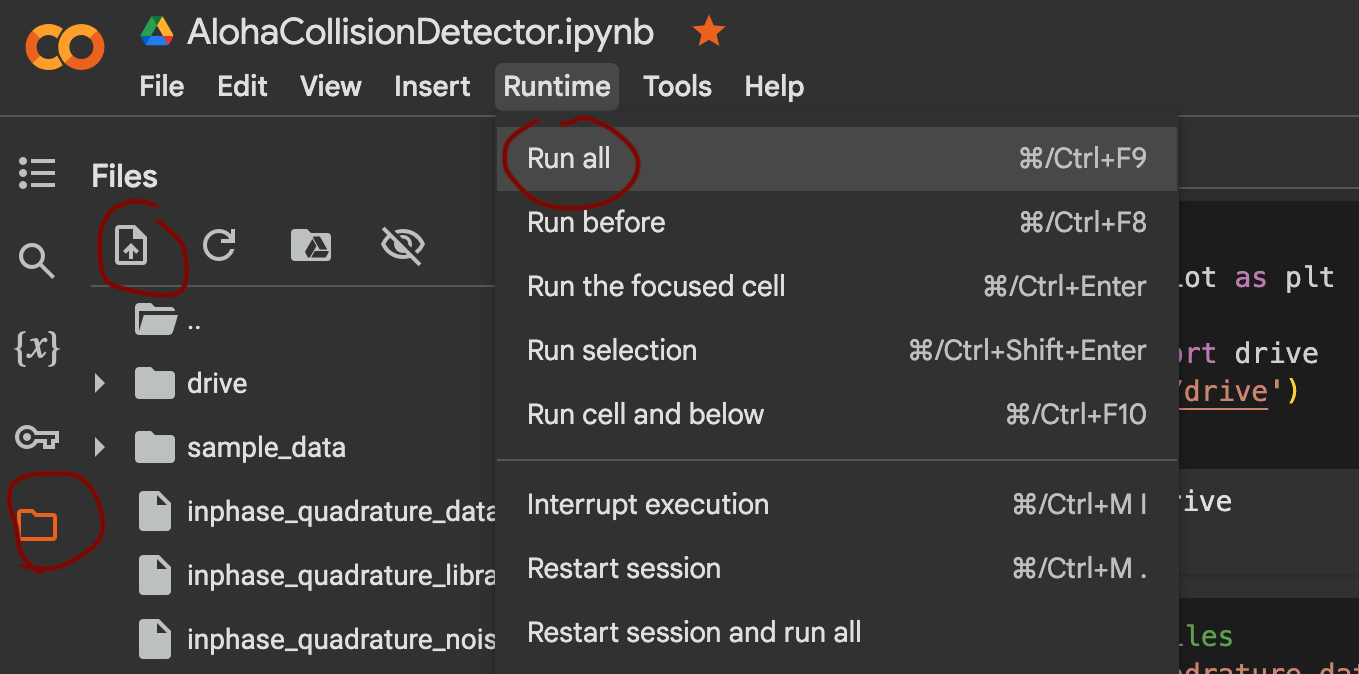
\includegraphics[width=0.5\textwidth]{fig_demo_upload}
\caption{Upload the files to Google Colab Python notebook and run the computational experiment.}
\label{fig:demo}
\end{figure}

\section{How to run the experiment}\label{sec:experiment}
\href{https://colab.research.google.com/drive/1wWEw8jcj8logartpd89VT_bX1jcP_VBb?usp=sharing}{Open the link to the Google Colab file} or copy the address to the browser:
{\footnotesize
\begin{verbatim}https://colab.research.google.com/drive/1wWEw8jcj8logartpd89VT_bX1jcP_VBb?usp=sharing\end{verbatim}}
\noindent
Press the ``Files'' icon on the left panel of Colab (the fifth from the top, below the key). Then press the ``Upload to session storage'' icon right below the word ``Files''.  From your local disk upload the files \textsf{inphase\_quadrature\_data.json}, \textsf{inphase\_quadrature\_noise.json}, and \textsf{inphase\_quadrature\_lib.npy}. The last one is attached along with this text. In the Colab menu click ``Runtime'' and select the item ``Run all''. After the first cell runs, Colab asks the access to the uploaded files. Press the button ``Continue'' each time to let the Google Colab access your Google Disk, \emph{there will be several consequent requests}. The experiment runs until the end. Figure~\ref{fig:demo} shows the orange ``Files'' icon and the ``Runtime'' menu open.\sloppy{}
%The link is %\textsf{https://colab.research.google.com/drive/1wWEw8jcj8logartpd89VT_bX1jcP_VBb?usp=sharing}




\section{Prominent applications}
The \cite{Katrutsa2017,Katrutsa2015}


and Future work and p
Prominent applications

I/Q data signal desoding in noise and cpmplex environment. 


TODO Further, we plan to use the methods of Independent Component Analysis and Blind Signal Separation in the time domain and frequency domain~\cite{Hyvaerinen2000,Elliott1999} of the I/Q data signal using a single reader (though this method requires at least two readers, and we do not count one reader has four antennas). 


\bibliographystyle{unsrt}
\bibliography{CollisionDetector}
\end{document}





